\documentclass[xetex,mathserif,serif]{beamer}
\usepackage{polyglossia}
\setdefaultlanguage[babelshorthands=true]{russian}
\usepackage{minted}
\usepackage{tabu}
\usepackage[11pt]{moresize}

\usepackage{textpos}
\setlength{\TPHorizModule}{1cm}
\setlength{\TPVertModule}{1cm}

\useoutertheme{infolines}

\usepackage{fontspec}
\setmainfont{FreeSans}
\newfontfamily{\russianfonttt}{FreeSans}

\definecolor{links}{HTML}{2A1B81}
\hypersetup{colorlinks,urlcolor=links}
\hypersetup{linkcolor=}

\newcommand{\attribution}[1] {
    \vspace{-5mm}\begin{flushright}\begin{scriptsize}\textcolor{gray}{\textcopyright\, #1}\end{scriptsize}\end{flushright}
}

\tabulinesep=0.7mm

\title{Лекция 8: Проектирование распределённых приложений}
\author[Юрий Литвинов]{Юрий Литвинов\\\small{\textcolor{gray}{y.litvinov@spbu.ru}}}

\date{19.05.2022}

\begin{document}
    
    \frame{\titlepage}

    \section{Введение}

    \begin{frame}
        \frametitle{Распределённые системы}
        \begin{itemize}
            \item Компоненты приложения находятся в компьютерной сети
            \item Взаимодействуют через обмен сообщениями
            \item Основное назначение --- работа с общими ресурсами
            \item Особенности
            \begin{itemize}
                \item Параллельная работа
                \item Независимые отказы
                \item Отсутствие единого времени
            \end{itemize}
        \end{itemize}
    \end{frame}

    \begin{frame}
        \frametitle{Частые заблуждения при проектировании распределённых систем}
        \begin{itemize}
            \item Сеть надёжна
            \item Задержка (latency) равна нулю
            \item Пропускная способность бесконечна
            \item Сеть безопасна
            \item Топология сети неизменна
            \item Администрирование сети централизовано
            \item Передача данных ``бесплатна''
            \item Сеть однородна
        \end{itemize}
    \end{frame}

    \section{Архитектура распределённых систем}

    \begin{frame}
        \frametitle{Виды взаимодействия}
        \begin{itemize}
            \item Межпроцессное взаимодействие
            \item Удалённые вызовы
            \begin{itemize}
                \item Протоколы вида ``запрос-ответ''
                \item Удалённые вызовы процедур (remote procedure calls, RPC)
                \item Удалённые вызовы методов (remote method invocation, RMI)
            \end{itemize}
            \item Неявное взаимодействие
            \begin{itemize}
                \item Групповое взаимодействие
                \item Модель ``издатель-подписчик''
                \item Очереди сообщений
                \item Распределённая общая память
            \end{itemize}
        \end{itemize}
    \end{frame}

    \begin{frame}
        \frametitle{Типичные архитектурные стили}
        \begin{itemize}
            \item Уровневая архитектура
            \begin{itemize}
                \item ОС
                \item Коммуникационная инфраструктура (Middleware)
                \item Приложения и сервисы
            \end{itemize}
            \item Клиент-сервер
            \begin{itemize}
                \item Тонкий клиент
                \item Бизнес-логика и данные --- на сервере
            \end{itemize}
            \item Трёхзвенная и N-уровневая архитектуры
            \begin{itemize}
                \item Бизнес-логику и работу с данными часто разделяют
            \end{itemize}
        \end{itemize}
    \end{frame}

    \section{Сетевое взаимодействие}

    \begin{frame}
        \frametitle{Модель OSI}
        \begin{center}
            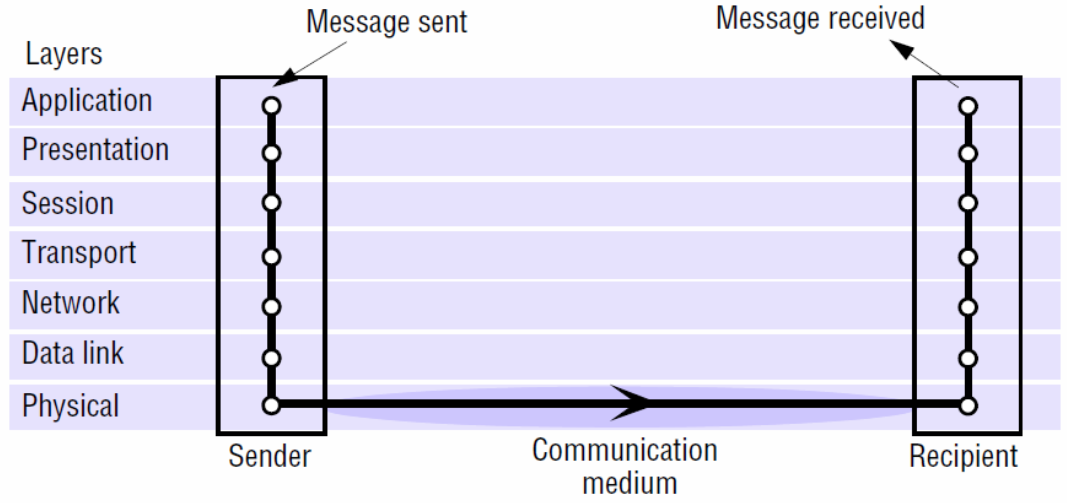
\includegraphics[width=0.8\textwidth]{osiStack.png}
        \end{center}
    \end{frame}

    \begin{frame}
        \frametitle{Стек протоколов TCP/IP}
        \begin{center}
            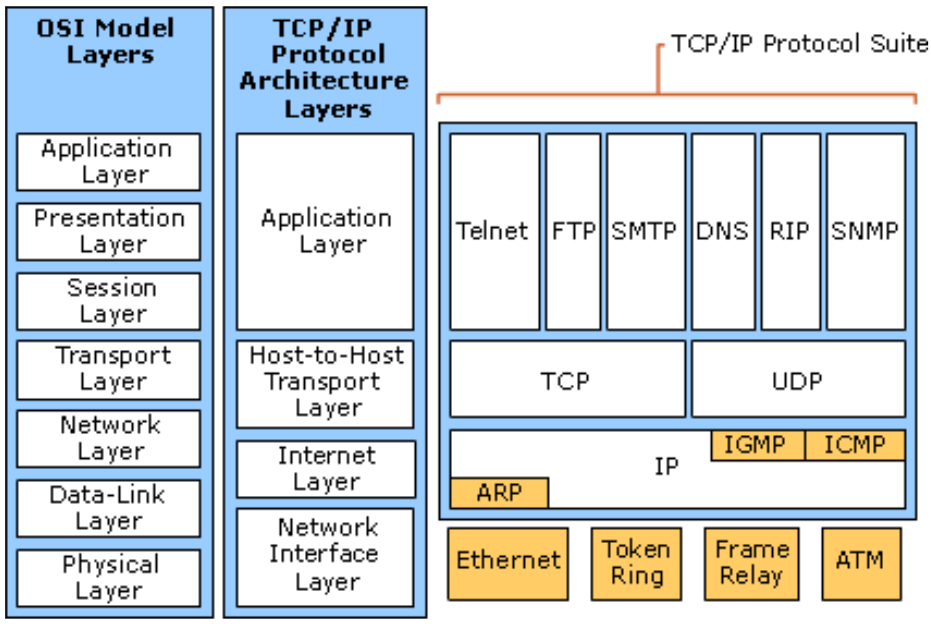
\includegraphics[width=0.8\textwidth]{tcpIpStack.png}
        \end{center}
    \end{frame}

    \section{Протоколы ``запрос-ответ''}

    \begin{frame}
        \frametitle{Протоколы ``запрос-ответ''}
        \begin{itemize}
            \item Запрос, действие, ответ
            \item Преимущественно синхронные вызовы
        \end{itemize}
        \begin{center}
            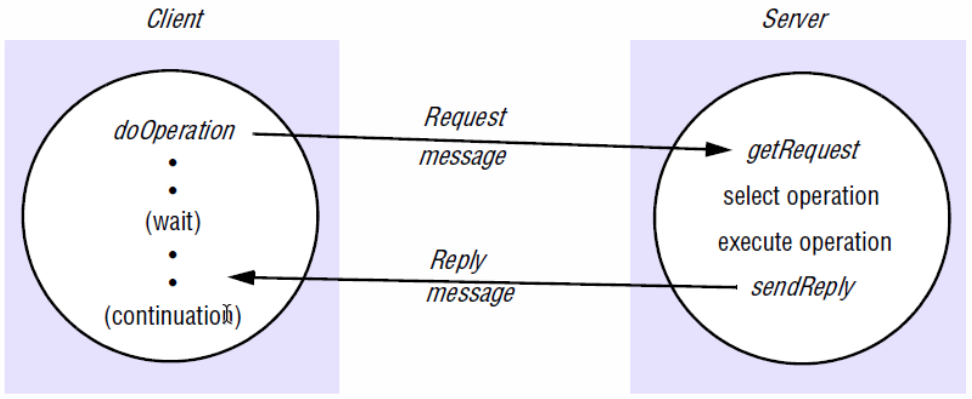
\includegraphics[width=0.8\textwidth]{requestReplyProtocols.png}
        \end{center}
    \end{frame}

    \begin{frame}
        \frametitle{``Запрос-ответ'' поверх UDP}
        \begin{itemize}
            \item[+] Уведомления не нужны
            \item[+] Установление соединения --- в два раза больше сообщений
            \item[+] Управление потоком не имеет смысла
            \item[-] Потери пакетов
            \begin{itemize}
                \item Таймаут + повторный запрос на уровне бизнес-логики
                \item Защита от повторного выполнения операции (хранение ``истории'')
                \item Новый запрос как подтверждение получения прошлого
            \end{itemize}
            \item[-] Неопределённый порядок пакетов
        \end{itemize}
    \end{frame}

    \begin{frame}
        \frametitle{``Запрос-ответ'' поверх TCP}
        \begin{itemize}
            \item[+] Использование потоков вместо набора пакетов
            \begin{itemize}
                \item Удобная отправка больших объёмов данных
                \item Один поток на всё взаимодействие
            \end{itemize}
            \item[+] Интеграция с потоками ОО-языков
            \item[+] Надёжность доставки
            \begin{itemize}
                \item Отсутствие необходимости проверок на уровне бизнес-логики
                \item Уведомления в пакетах с ответом
                \item Упрощение реализации
            \end{itemize}
            \item[-] Тяжеловесность коммуникации
        \end{itemize}
    \end{frame}

    \section{RPC}

    \begin{frame}
        \frametitle{RPC}
        \begin{center}
            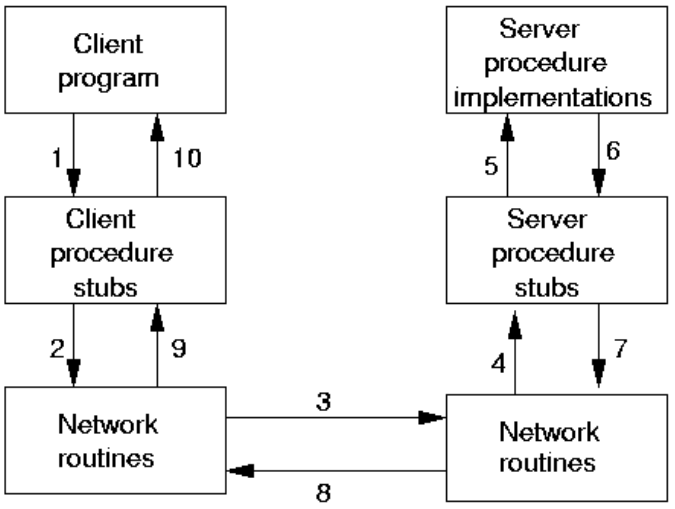
\includegraphics[width=0.6\textwidth]{rpc.png}
        \end{center}
    \end{frame}

    \begin{frame}
        \frametitle{Прозрачность RPC-вызовов}
        \begin{itemize}
            \item Изначальная цель --- максимальная похожесть на обычные вызовы
            \begin{itemize}
                \item Location and access transparency
            \end{itemize}
            \item Удалённые вызовы более уязвимы к отказам
            \begin{itemize}
                \item Нужно понимать разницу между отказом сети и отказом сервиса
                \begin{itemize}
                    \item Exponential backoff
                \end{itemize}
                \item Клиенты должны знать о задержках при передаче данных
                \begin{itemize}
                    \item Возможность прервать вызов
                \end{itemize}
            \end{itemize}
            \item Явная маркировка удалённых вызовов?
            \begin{itemize}
                \item Прозрачность синтаксиса
                \item Явное отличие в интерфейсах
                \begin{itemize}
                    \item Указание сематики вызова
                \end{itemize}
            \end{itemize}
        \end{itemize}
    \end{frame}

    \section{RMI}

    \begin{frame}
        \frametitle{Удалённые вызовы методов (RMI)}
        \begin{itemize}
            \item Продолжение идей RPC
            \begin{itemize}
                \item Программирование через интерфейсы
                \item Работа поверх протоколов ``запрос-ответ''
                \item At-least-once или at-most-once семантика вызовов
                \item Прозрачность синтаксиса вызовов
            \end{itemize}
            \item Особенности ОО-программ
            \begin{itemize}
                \item Наследование, полиморфизм
                \item Передача параметров по ссылкам
                \item Исключения
                \item Распределённая сборка мусора
            \end{itemize}
        \end{itemize}
    \end{frame}

    \section{protobuf}

    \begin{frame}
        \frametitle{Protocol buffers}
        \framesubtitle{protobuf}
        \begin{itemize}
            \item Механизм сериализации-десериализации данных
            \item Компактное бинарное представление
            \item Декларативное описание формата данных, генерация кода для языка программирования
            \begin{itemize}
                \item Поддерживается Java, Python, Objective-C, C++, Go, JavaNano, Ruby, C\#
            \end{itemize}
            \item Бывает v2 и v3, с некоторыми синтаксическими отличиями
            \item Хитрый протокол передачи, \url{https://developers.google.com/protocol-buffers/docs/encoding}
            \begin{itemize}
                \item До 10 раз компактнее XML 
            \end{itemize}
        \end{itemize}
    \end{frame}

    \begin{frame}[fragile]
        \frametitle{Пример}
        Файл .proto:
        \begin{minted}{protobuf}
message Person {
  required string name = 1;
  required int32 id = 2;
  optional string email = 3;
}
        \end{minted}
        \vspace{2mm}
        Файл .java:
        \begin{minted}{java}
Person john = Person.newBuilder()
    .setId(1234)
    .setName("John Doe")
    .setEmail("jdoe@example.com")
    .build();
output = new FileOutputStream(args[0]);
john.writeTo(output);
        \end{minted}
    \end{frame}

    \section{gRPC}

    \begin{frame}
        \frametitle{gRPC}
        \begin{columns}
            \begin{column}{0.6\textwidth}
                \begin{itemize}
                    \item средство для удалённого вызова (RPC)
                    \item Работает поверх protobuf
                    \item Разрабатывается Google
                    \item Поддерживает C++, Java, Objective-C, Python, Ruby, Go, C\#, Node.js
                \end{itemize}
            \end{column}
            \begin{column}{0.4\textwidth}
                \begin{center}
                    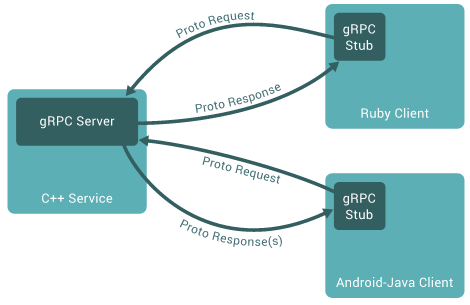
\includegraphics[width=\textwidth]{grpc.png}
                \end{center}
            \end{column}
        \end{columns}
    \end{frame}

    \begin{frame}[fragile]
        \frametitle{Технические подробности}
        \begin{itemize}
            \item Сервисы описываются в том же .proto-файле, что и протокол protobuf-а
            \item В качестве типов параметров и результатов --- message-и protobuf-а
        \end{itemize}
        \begin{minted}{protobuf}
service RouteGuide {
  rpc GetFeature(Point) returns (Feature) {}
  rpc ListFeatures(Rectangle) returns (stream Feature) {}
  rpc RecordRoute(stream Point) returns (RouteSummary) {}
  rpc RouteChat(stream RouteNote) returns (stream RouteNote) {}
}
        \end{minted}
        \begin{itemize}
            \item Сборка --- плагином grpc к protoc
        \end{itemize}
\end{frame}

    \begin{frame}[fragile]
        \frametitle{Реализация сервиса на Java}
        \begin{scriptsize}
            \begin{minted}{java}
private static class RouteGuideService extends RouteGuideGrpc.RouteGuideImplBase {
    ...
    @Override
    public void getFeature(Point request, StreamObserver<Feature> responseObserver) {
      responseObserver.onNext(checkFeature(request));
      responseObserver.onCompleted();
    }

    @Override
    public void listFeatures(Rectangle request, StreamObserver<Feature> responseObserver) {
      for (Feature feature : features) {
        ...
        int lat = feature.getLocation().getLatitude();
        int lon = feature.getLocation().getLongitude();
        if (lon >= left && lon <= right && lat >= bottom && lat <= top) {
          responseObserver.onNext(feature);
        }
      }
      responseObserver.onCompleted();
    }
            \end{minted}
        \end{scriptsize}
    \end{frame}

    \begin{frame}[fragile]
        \frametitle{Реализация сервиса на Java (2)}
        \begin{scriptsize}
            \begin{minted}{java}
    @Override
    public StreamObserver<RouteNote> routeChat(
            final StreamObserver<RouteNote> responseObserver) {
      return new StreamObserver<RouteNote>() {
        @Override
        public void onNext(RouteNote note) {
          List<RouteNote> notes = getOrCreateNotes(note.getLocation());
          for (RouteNote prevNote : notes.toArray(new RouteNote[0])) {
            responseObserver.onNext(prevNote);
          }
          notes.add(note);
        }
        @Override
        public void onError(Throwable t) {
          logger.log(Level.WARNING, "routeChat cancelled");
        }
        @Override
        public void onCompleted() {
          responseObserver.onCompleted();
        }
      };
    }
            \end{minted}
        \end{scriptsize}
    \end{frame}

    \begin{frame}[fragile]
        \frametitle{Реализация клиента на Java (1)}
        \begin{scriptsize}
            \begin{minted}{java}
public RouteGuideClient(String host, int port) {
    this(ManagedChannelBuilder.forAddress(host, port).usePlaintext(true));
}

public RouteGuideClient(ManagedChannelBuilder<?> channelBuilder) {
    channel = channelBuilder.build();
    blockingStub = RouteGuideGrpc.newBlockingStub(channel);
    asyncStub = RouteGuideGrpc.newStub(channel);
}
            \end{minted}
        \end{scriptsize}
    \end{frame}

    \begin{frame}[fragile]
        \frametitle{Реализация клиента на Java (2)}
        \begin{scriptsize}
            \begin{minted}{java}
public void getFeature(int lat, int lon) {
    Point request = Point.newBuilder().setLatitude(lat).setLongitude(lon).build();
    Feature feature;
    try {
        feature = blockingStub.getFeature(request);
    } catch (StatusRuntimeException e) {
        warning("RPC failed: {0}", e.getStatus());
        return;
    }
    if (RouteGuideUtil.exists(feature)) {
        info("Found feature called \"{0}\" at {1}, {2}",
            feature.getName(),
            RouteGuideUtil.getLatitude(feature.getLocation()),
            RouteGuideUtil.getLongitude(feature.getLocation()));
    } else {
        info("Found no feature at {0}, {1}",
            RouteGuideUtil.getLatitude(feature.getLocation()),
            RouteGuideUtil.getLongitude(feature.getLocation()));
    }
}
            \end{minted}
        \end{scriptsize}
    \end{frame}

    \section{Веб-сервисы}

    \begin{frame}
        \frametitle{Веб-сервисы}
        \begin{itemize}
            \item Перенос специализации клиент-сервера в web
            \item Cложные приложения как интеграция веб-сервисов
            \item HTTP-запрос для выполнения команды
            \begin{itemize}
                \item Aсинхронное взаимодействие
                \item Ответ-запрос
                \item Событийные схемы
            \end{itemize}
            \item XML или JSON как основной формат сообщений
            \begin{itemize}
                \item SOAP/WSDL/UDDI
                \item XML-RPC
                \item REST
            \end{itemize}
        \end{itemize}
    \end{frame}

    \section{SOAP}

    \begin{frame}
        \frametitle{SOAP-ориентированные сервисы}
        \begin{columns}
            \begin{column}{0.6\textwidth}
                \begin{itemize}
                    \item Simple Object Access Protocol
                    \item Web Services Description Language
                    \item Universal Discovery, Description and Integration
                \end{itemize}
            \end{column}
            \begin{column}{0.4\textwidth}
                \begin{center}
                    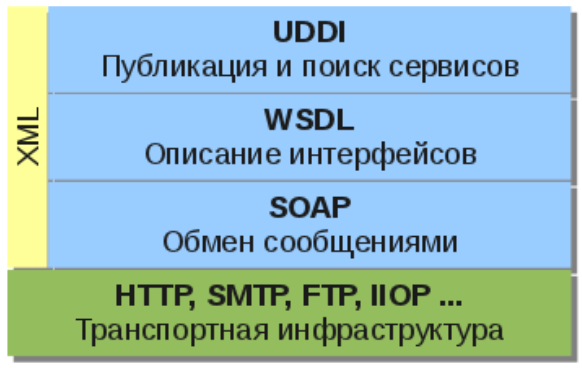
\includegraphics[width=\textwidth]{soap.png}
                \end{center}
            \end{column}
        \end{columns}
    \end{frame}

    \begin{frame}[fragile]
        \frametitle{SOAP-сообщение}
        \begin{small}
            \begin{minted}{xml}
<env:Envelope xmlns:env="http://www.w3.org/2003/05/soap-envelope">
    <env:Header>
        <n:alertcontrol xmlns:n="http://example.org/alertcontrol">
            <n:priority>1</n:priority>
            <n:expires>2001-06-22T14:00:00-05:00</n:expires>
        </n:alertcontrol>
    </env:Header>
    <env:Body>
        <m:alert xmlns:m="http://example.org/alert">
            <m:msg>Get up at 6:30 AM</m:msg>
        </m:alert>
    </env:Body>
</env:Envelope>
            \end{minted}
        \end{small}
    \end{frame}

    \begin{frame}[fragile]
        \frametitle{WSDL-описание}
        \begin{small}
            \begin{minted}{xml}
<message name="getTermRequest">
    <part name="term" type="xs:string"/>
</message>

<message name="getTermResponse">
    <part name="value" type="xs:string"/>
</message>

<portType name="glossaryTerms">
    <operation name="getTerm">
        <input message="getTermRequest"/>
        <output message="getTermResponse"/>
    </operation>
</portType>
            \end{minted}
        \end{small}
    \end{frame}

    \begin{frame}
        \frametitle{Достоинства SOAP-based сервисов}
        \begin{itemize}
            \item Автоматический режим описания сервисов
            \item Автоматическая поддержка описаний SOAP-клиентом
            \item Автоматическая валидация сообщений
            \begin{itemize}
                \item Валидность xml
                \item Проверка по схеме
                \item Проверка SOAP-сервером
            \end{itemize}
            \item Работа через HTTP
            \begin{itemize}
                \item Хоть через обычный GET
            \end{itemize}
        \end{itemize}
    \end{frame}

    \section{WCF}

    \begin{frame}
        \frametitle{Пример: WCF}
        \begin{itemize}
            \item Платформа для создания веб-сервисов
            \item Часть .NET Framework, начиная с 3.0
            \item Умеет WSDL, SOAP и т.д., очень конфигурируема
            \item Автоматическая генерация заглушек на стороне клиента
            \item ABCs of WCF:
            \begin{itemize}
                \item Address
                \item Binding
                \item Contract
            \end{itemize}
        \end{itemize}
        \begin{center}
            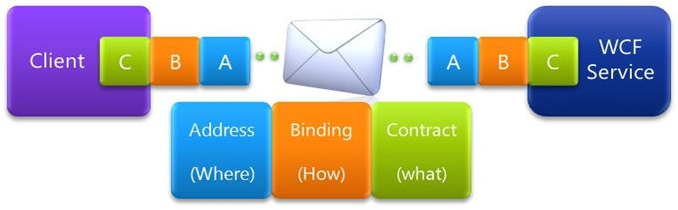
\includegraphics[width=0.6\textwidth]{wcf.png}
            \attribution{\url{http://www.c-sharpcorner.com}}
        \end{center}
    \end{frame}

    \begin{frame}[fragile]
        \frametitle{Пример, описание контракта}
        \begin{small}
            \begin{minted}{csharp}
[ServiceContract(Namespace = "http://Microsoft.ServiceModel.Samples")]  
public interface ICalculator  
{
    [OperationContract]
    double Add(double n1, double n2);

    [OperationContract]
    double Subtract(double n1, double n2);

    [OperationContract]
    double Multiply(double n1, double n2);

    [OperationContract]
    double Divide(double n1, double n2);
}
            \end{minted}
        \end{small}
    \end{frame}

    \begin{frame}[fragile]
        \frametitle{Пример, реализация контракта}
        \begin{small}
            \begin{minted}{csharp}
public class CalculatorService : ICalculator  
{
    public double Add(double n1, double n2)
        => n1 + n2;  

    public double Subtract(double n1, double n2)
        => n1 - n2

    public double Multiply(double n1, double n2)  
        => n1 * n2;

    public double Divide(double n1, double n2)  
        => n1 / n2;
}
            \end{minted}
        \end{small}
    \end{frame}

    \begin{frame}[fragile]
        \frametitle{Пример, self-hosted service}
        \begin{scriptsize}
            \begin{minted}{csharp}
static void Main(string[] args) 
{
    Uri baseAddress = new Uri("http://localhost:8000/ServiceModelSamples/Service");
    ServiceHost selfHost = new ServiceHost(typeof(CalculatorService), baseAddress);

    try {
        selfHost.AddServiceEndpoint(typeof(ICalculator), new WSHttpBinding(), "CalculatorService");

        ServiceMetadataBehavior smb = new ServiceMetadataBehavior();
        smb.HttpGetEnabled = true;
        selfHost.Description.Behaviors.Add(smb);

        selfHost.Open();
        Console.WriteLine("The service is ready. Press <ENTER> to terminate service.");
        Console.ReadLine();

        selfHost.Close();  
    } catch (CommunicationException ce) {
        Console.WriteLine($"An exception occurred: {ce.Message}");
        selfHost.Abort();
    }
}
            \end{minted}
        \end{scriptsize}
    \end{frame}

    \begin{frame}[fragile]
        \frametitle{Пример, клиент}
        \begin{itemize}
            \item Генерация заглушки: 
                \begin{scriptsize}
                    \begin{minted}{text}
svcutil.exe /language:cs /out:generatedProxy.cs /config:app.config^
    http://localhost:8000/ServiceModelSamples/service
                    \end{minted}
                \end{scriptsize}
            \item Клиент:
                \begin{footnotesize}
                    \begin{minted}{csharp}
static void Main(string[] args)
{
    CalculatorClient client = new CalculatorClient();

    double value1 = 100.00D;
    double value2 = 15.99D;
    double result = client.Add(value1, value2);
    Console.WriteLine($"Add({value1},{value2}) = {result}");

    client.Close();
}
                    \end{minted}
                \end{footnotesize}
        \end{itemize}
    \end{frame}

    \begin{frame}[fragile]
        \frametitle{Пример, конфигурация клиента}
        \begin{ssmall}
            \begin{minted}{xml}
<?xml version="1.0" encoding="utf-8" ?>  
<configuration>  
    <startup>   
      <!-- specifies the version of WCF to use-->  
        <supportedRuntime version="v4.0" sku=".NETFramework,Version=v4.5,Profile=Client" />  
    </startup>  
    <system.serviceModel>  
        <bindings>  
            <!-- Uses wsHttpBinding-->  
            <wsHttpBinding>  
                <binding name="WSHttpBinding_ICalculator" />  
            </wsHttpBinding>  
        </bindings>  
        <client>  
            <!-- specifies the endpoint to use when calling the service -->  
            <endpoint address="http://localhost:8000/ServiceModelSamples/Service/CalculatorService"  
                binding="wsHttpBinding" bindingConfiguration="WSHttpBinding_ICalculator"  
                contract="ServiceReference1.ICalculator" name="WSHttpBinding_ICalculator">  
                <identity>  
                    <userPrincipalName value="migree@redmond.corp.microsoft.com" />  
                </identity>  
            </endpoint>  
        </client>  
    </system.serviceModel>  
</configuration>
            \end{minted}
        \end{ssmall}
    \end{frame}

    \section{Очереди сообщений}

    \begin{frame}
        \frametitle{Очереди сообщений}
        \begin{itemize}
            \item Используются для гарантированной доставки сообщений
            \begin{itemize}
                \item Даже если отправитель и получатель доступны в разное время
                \item Локальное хранилище сообщений на каждом устройстве
            \end{itemize}
            \item Реализуют модель ``издатель-подписчик'', но могут работать и в режиме ``точка-точка''
            \item Как правило, имеют развитые возможности маршрутизации, фильтрации и преобразования сообщений
            \begin{itemize}
                \item Разветвители, агрегаторы, преобразователи порядка
            \end{itemize}
        \end{itemize}
    \end{frame}

    \section{RabbitMQ}

    \begin{frame}
        \frametitle{RabbitMQ}
        \begin{itemize}
            \item Сервер и клиенты системы надёжной передачи сообщений
            \begin{itemize}
                \item Сообщение посылается на сервер и хранится там, пока его не заберут
                \item Продвинутые возможности по маршрутизации сообщений
            \end{itemize}
            \item Реализует протокол AMQP (Advanced Message Queuing Protocol), но может использовать и другие протоколы
            \item Сервер написан на Erlang, клиентские библиотеки доступны для практически чего угодно
        \end{itemize}
        \begin{textblock}{3}(8,0)
            
\includegraphics[width=\textwidth]{rabbitmqLogo.png}
        \end{textblock}
    \end{frame}

    \begin{frame}[fragile]
        \frametitle{Пример, отправитель}
        \begin{ssmall}
            \begin{minted}{csharp}
using System;
using RabbitMQ.Client;
using System.Text;

class Send
{
    public static void Main()
    {
        var factory = new ConnectionFactory() { HostName = "localhost" };
        using (var connection = factory.CreateConnection())
        {
            using (var channel = connection.CreateModel())
            {
                channel.QueueDeclare(queue: "hello", durable: false, exclusive: false,
                                     autoDelete: false, arguments: null);

                string message = "Hello World!";
                var body = Encoding.UTF8.GetBytes(message);

                channel.BasicPublish(exchange: "", routingKey: "hello",
                                     basicProperties: null, body: body);
            }
        }
    }
}
            \end{minted}
        \end{ssmall}
    \end{frame}

    \begin{frame}[fragile]
        \frametitle{Пример, получатель}
        \begin{ssmall}
            \begin{minted}{csharp}
using RabbitMQ.Client;
using RabbitMQ.Client.Events;
using System;
using System.Text;

class Receive
{
    public static void Main()
    {
        var factory = new ConnectionFactory() { HostName = "localhost" };
        using (var connection = factory.CreateConnection())
        using (var channel = connection.CreateModel())
        {
            channel.QueueDeclare(queue: "hello", durable: false, exclusive: false, autoDelete: false, arguments: null);

            var consumer = new EventingBasicConsumer(channel);
            consumer.Received += (model, ea) =>
            {
                var body = ea.Body;
                var message = Encoding.UTF8.GetString(body);
                Console.WriteLine(" [x] Received {0}", message);
            };
            channel.BasicConsume(queue: "hello", autoAck: true, consumer: consumer);
        }
    }
}
            \end{minted}
        \end{ssmall}
    \end{frame}

    \section{REST}

    \begin{frame}
        \frametitle{Representational State Transfer (REST)}
        \begin{itemize}
            \item Модель клиент-сервер
            \item Отсутствие состояния
            \item Кэширование
            \item Единообразие интерфейса
            \item Слои
        \end{itemize}
    \end{frame}

    \begin{frame}
        \frametitle{Интерфейс сервиса}
        \begin{itemize}
            \item Коллекции
            \begin{itemize}
                \item \url{http://api.example.com/resources/}
            \end{itemize}
            \item Элементы
            \begin{itemize}
                \item \url{http://api.example.com/resources/item/17}
            \end{itemize}
            \item HTTP-методы
            \begin{itemize}
                \item GET
                \item PUT
                \item POST
                \item DELETE
            \end{itemize}
            \item Передача параметров прямо в URL
            \begin{itemize}
                \item \url{http://api.example.com/resources?user=me&access_token=ASFQF}
            \end{itemize}
        \end{itemize}
    \end{frame}

    \begin{frame}
        \frametitle{Пример, Google Drive REST API}
        \begin{itemize}
            \item GET https://www.googleapis.com/drive/v2/files --- список всех файлов
            \item GET https://www.googleapis.com/drive/v2/files/fileId --- метаданные файла по его Id
            \item POST https://www.googleapis.com/upload/drive/v2/files — загрузить новый файл
            \item PUT https://www.googleapis.com/upload/drive/v2/files/fileId --- обновить файл
            \item DELETE https://www.googleapis.com/drive/v2/files/fileId --- удалить файл
        \end{itemize}
    \end{frame}

    \begin{frame}
        \frametitle{Достоинства}
        \begin{itemize}
            \item Надёжность
            \item Производительность
            \item Масштабируемость
            \item Прозрачность системы взаимодействия
            \item Простота интерфейсов
            \item Портативность компонентов
            \item Лёгкость внесения изменений
        \end{itemize}
    \end{frame}

    \section{Микросервисы}

    \begin{frame}
        \frametitle{Микросервисы}
        \begin{itemize}
            \item Набор небольших сервисов
            \begin{itemize}
                \item Разные языки и технологии
            \end{itemize}
            \item Каждый в собственном процессе
            \begin{itemize}
                \item Независимое развёртывание
                \item Децентрализованное управление
            \end{itemize}
            \item Легковесные коммуникации
        \end{itemize}
    \end{frame}

    \begin{frame}
        \frametitle{Монолитные приложения}
        \begin{itemize}
            \item Большой и сложный MVC
            \item Единый процесс разработки и стек технологий
            \item Сложная архитектура
            \item Сложно масштабировать
            \item Сложно вносить изменения
        \end{itemize}
    \end{frame}

    \begin{frame}
        \frametitle{Разбиение на сервисы}
        \begin{center}
            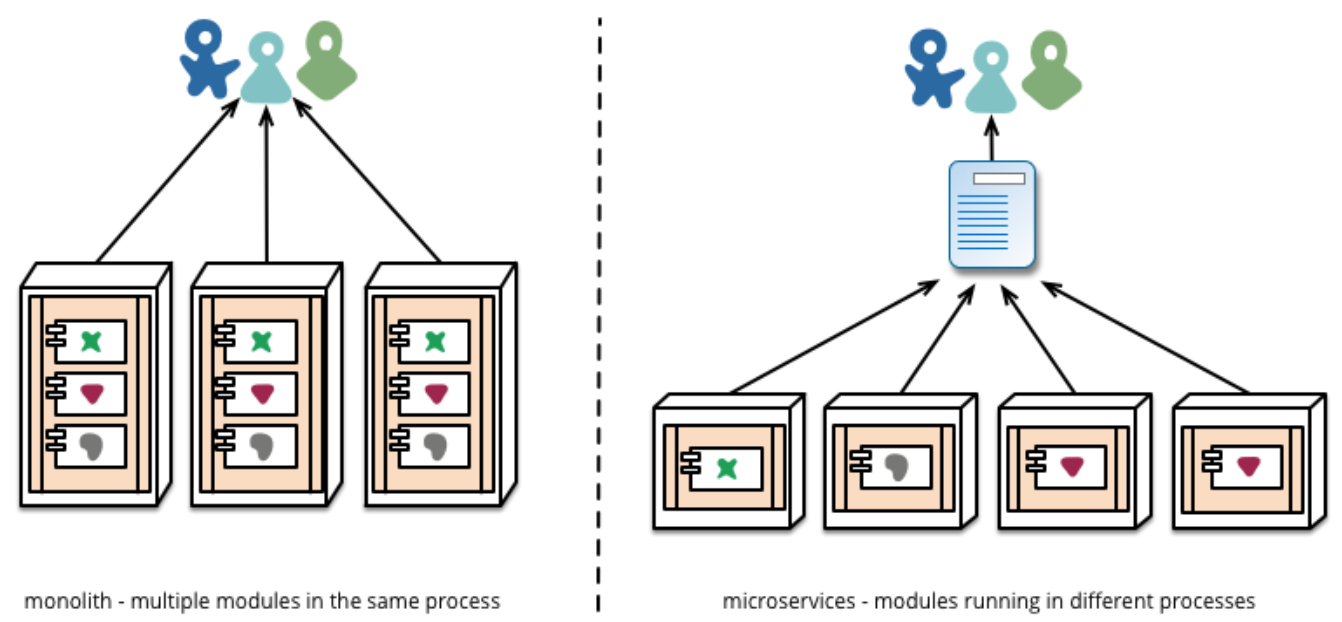
\includegraphics[width=\textwidth]{microservices.png}
        \end{center}
    \end{frame}

    \begin{frame}
        \frametitle{Основные проблемы}
        \begin{itemize}
            \item Сложности выделения границ сервисов
            \item Перенос логики на связи между сервисами
            \begin{itemize}
                \item Большой обмен данными
                \item Нетривиальные зависимости
            \end{itemize}
            \item Нетривиальная инфраструктура
            \item Нетривиальная переиспользуемость кода
        \end{itemize}
    \end{frame}

    \section{Peer-to-peer}

    \begin{frame}
        \frametitle{Архитектура Peer-to-Peer}
        \begin{itemize}
            \item Децентрализованный и самоорганизующийся сервис
            \item Динамическая балансировка нагрузки
            \begin{itemize}
                \item Вычислительные ресурсы
                \item Хранилища данных
            \end{itemize}
            \item Динамическое изменение состава участников
        \end{itemize}
    \end{frame}

    \begin{frame}
        \frametitle{Skype: Overlayed P2P}
        \begin{center}
            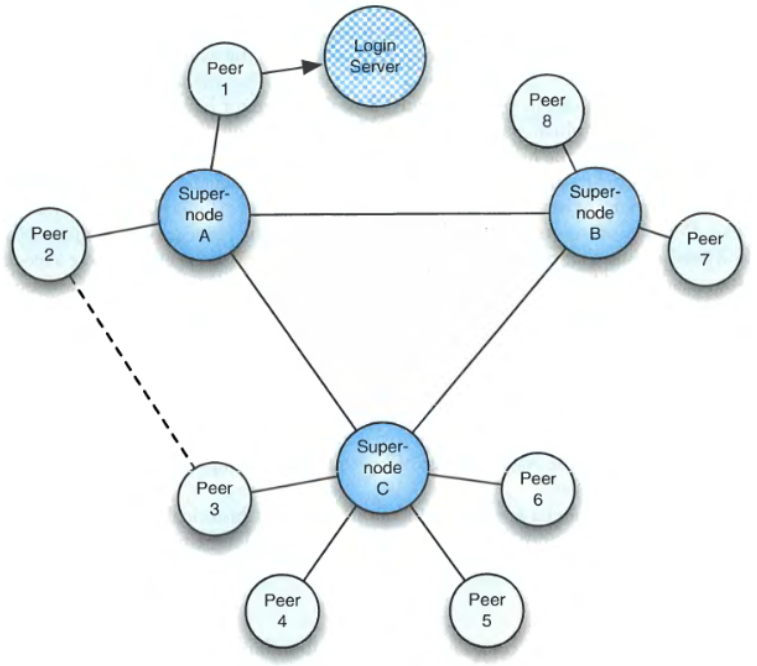
\includegraphics[width=0.6\textwidth]{skype.png}
        \end{center}
    \end{frame}

    \begin{frame}
        \frametitle{BitTorrent : Resource Trading P2P}
        \begin{itemize}
            \item Обмен сегментами
            \item Поиск не входит в протокол
            \item Трекеры
            \item Метаданные
            \item Управление приоритетами
            \item Бестрекерная реализация
        \end{itemize}
    \end{frame}

\end{document}
